{\bf Dynamically adaptive grid.}
Our dynamically adaptive grid is characterised by two ingredients: mesh
refinement control and inter-grid particle treatment.
In \texttt{touchVertexFirstTime}, our code analyses what the smallest diameter
of all the particles held by the vertex is.
If this diameter is smaller than $1/3$ of the mesh width corresponding to the
vertex's level, then the region around the vertex is refined.
If we run into a vertex, we check whether there are any spatially coinciding
vertices in the tree on a coarser level.
If such vertices do exist, we run through all of their particles and move them
one level down if the diameter permits.
The scheme successively drops the particles down the grid hierarchies.

\begin{figure}
 \begin{center}
  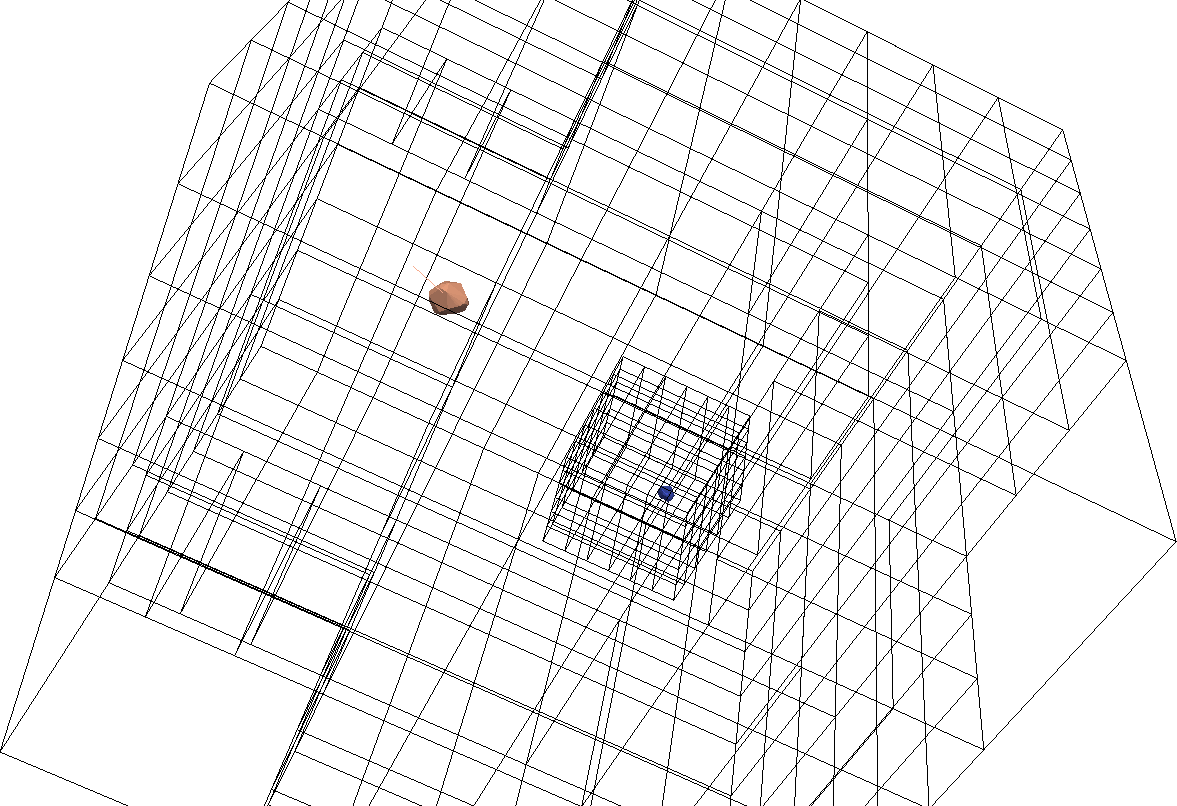
\includegraphics[width=0.4\textwidth]{experiments/two-bodies/visualisation/adaptive-grid00.png}
  \hspace{1.1cm}
  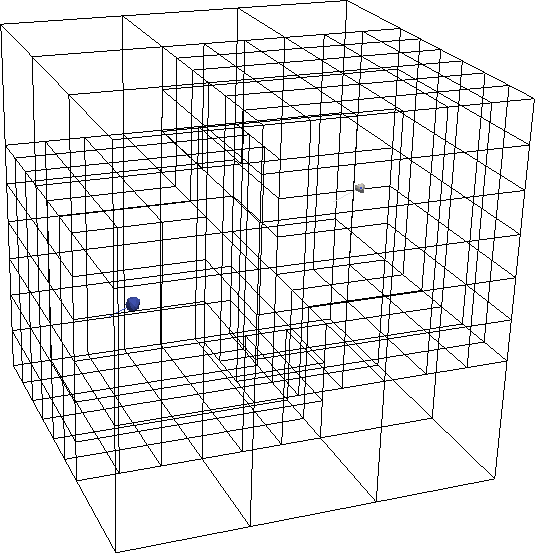
\includegraphics[width=0.25\textwidth]{experiments/two-bodies/visualisation/reluctant-adaptive-grid00.png}
  \\
  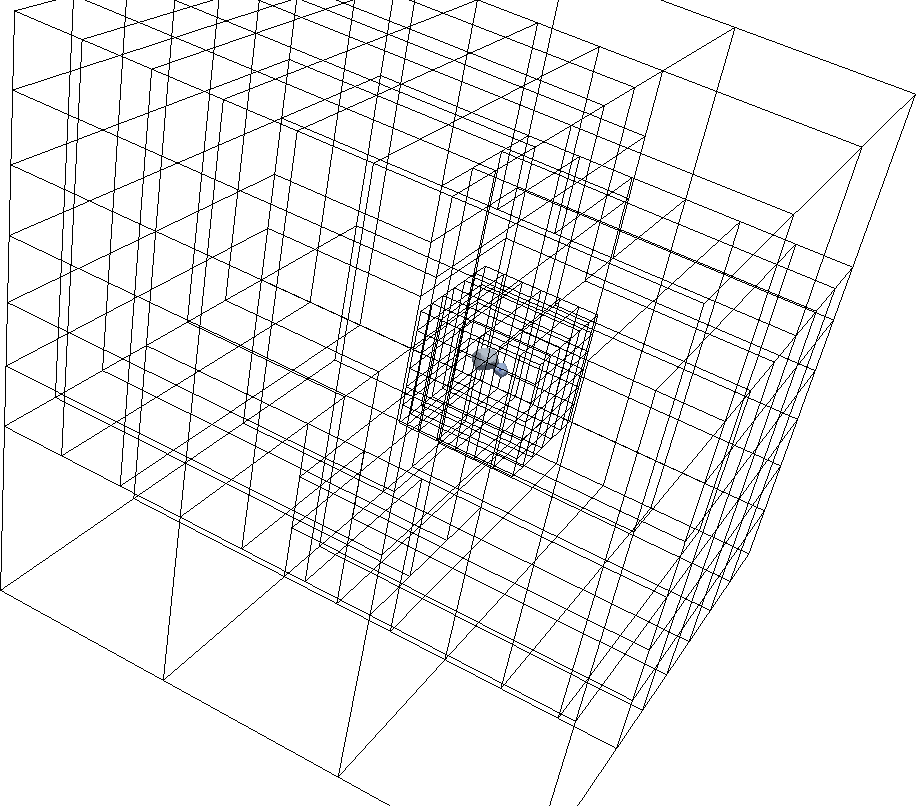
\includegraphics[width=0.3\textwidth]{experiments/two-bodies/visualisation/adaptive-grid02.png}
  \hspace{1.1cm}
  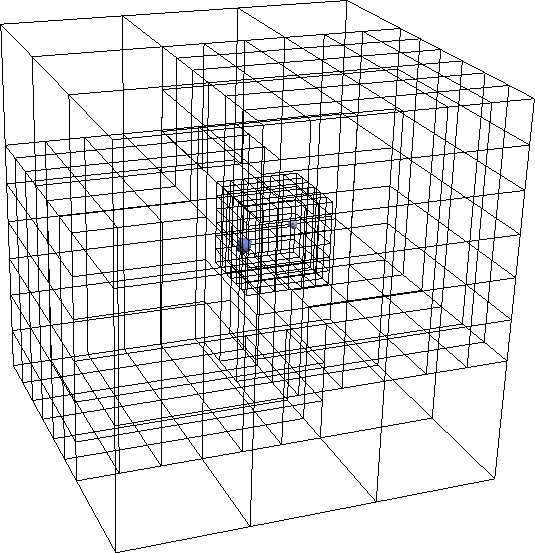
\includegraphics[width=0.3\textwidth]{experiments/two-bodies/visualisation/reluctant-adaptive-grid02.png}
% 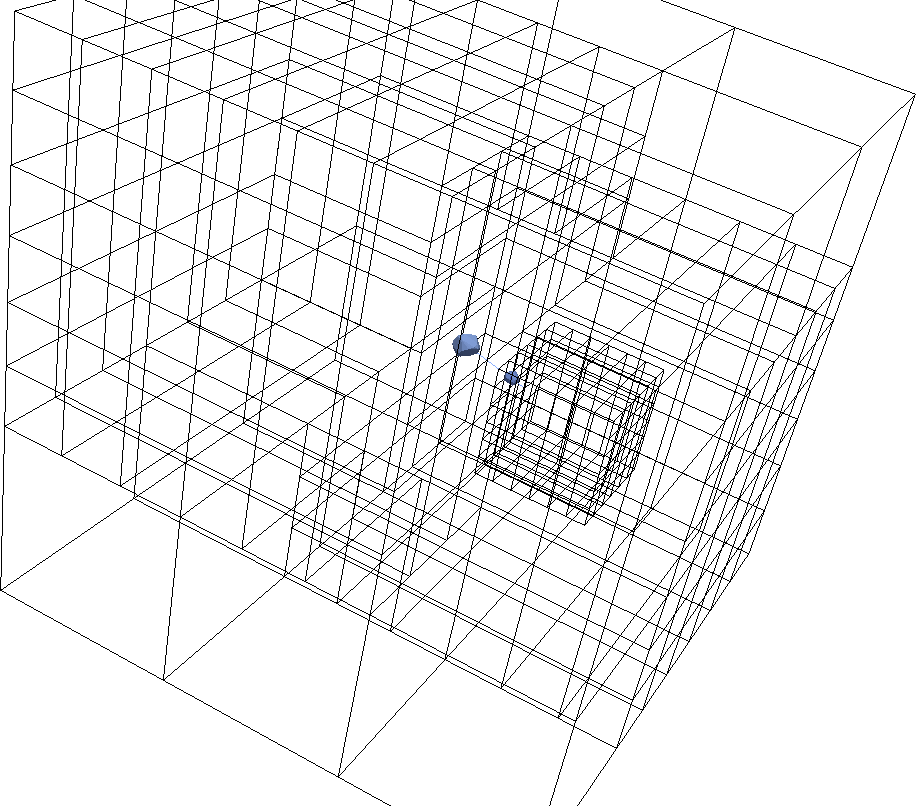
\includegraphics[width=0.3\textwidth]{experiments/two-bodies/visualisation/adaptive-grid01.png}
%   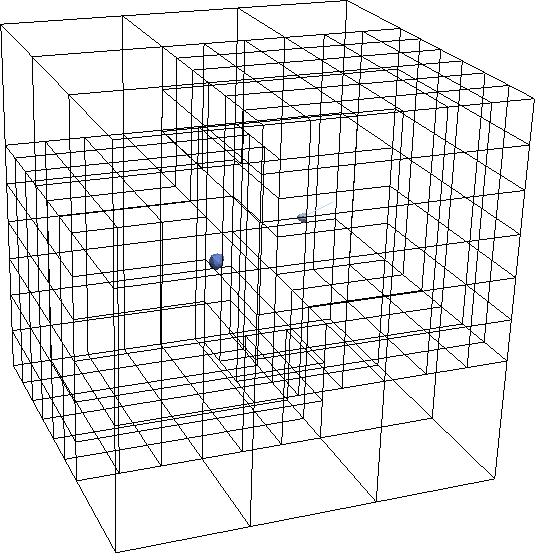
\includegraphics[width=0.3\textwidth]{experiments/two-bodies/visualisation/reluctant-adaptive-grid01.png}\\
%   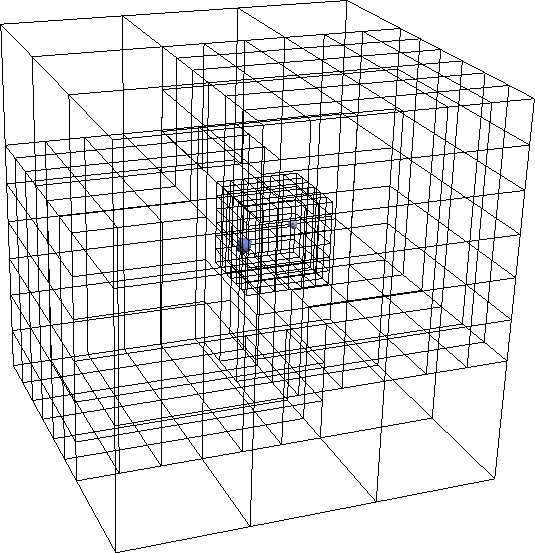
\includegraphics[width=0.3\textwidth]{experiments/two-bodies/visualisation/reluctant-adaptive-grid02.png}
%   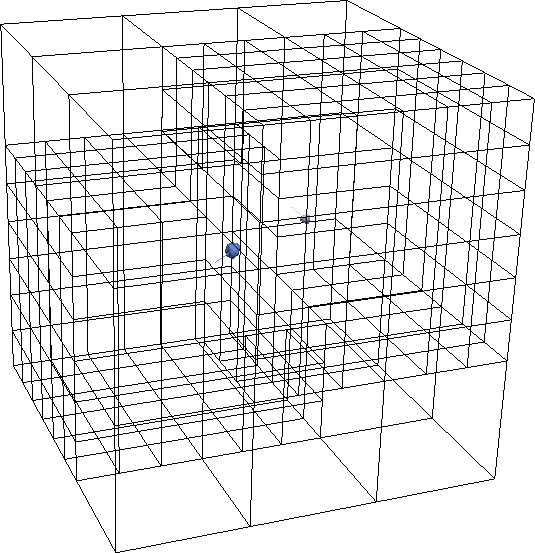
\includegraphics[width=0.3\textwidth]{experiments/two-bodies/visualisation/reluctant-adaptive-grid03.png}\\
 \end{center}
 \caption{
   Two particles crash into each other.
   The adaptive grid refining around each particle while its diameter
   constrains the mesh size (left column).
   The reluctant adaptive grid works with a coarser resolution as long
   as particles are far away from each other (right column).
   Just before they collide, the grid is refined and particles are dropped down
   the resolution levels.
 }
 \label{figure:adaptive-vs-reluctant-grid}
\end{figure}

We define two multiscale relationships between vertices (Figure
\ref{figure:collision-cube}).
A vertex $a$ is a child of a vertex $b$ if all adjacent cells of $a$ are
children of adjacent cells of $b$. $b$ is the parent vertex of $a$.
A vertex $a$ is a descendant of $b$ if at least one adjacent cell of $a$ is a
child of an adjacent cell of $b$. $b$ is an ancestor of $a$.
If we delete a vertex $a$ that holds particles, its particles are moved to the
next coarser level and assigned there to the nearest parent of $a$.
Each vertex holds a boolean marker that is set $\bot $ before the vertex is
read for the first time.
If a vertex holds a particle, all the markers of the vertices where it is a
descendent from are set to $\top$.
If a vertex whose adjacent cells all are refined holds $\bot$ at the end of the
multiscale traversal, we coarsen these refined adjacent cells.
We rely on a top-down tree traversal.
The refinement/coarsening procedure then can be evaluated on-the-fly.
It equals an analysed tree grammar \cite{Knuth71}.

For the multiscale contact detection, we extend the list of particles associated
to a vertex. 
There is the list of actually held particles and a list of virtual particles. 
We run through the grid top down, i.e.~a vertex always is read for the first
time before any of its descendants, and clear virtual particle list first.
Then, we add all particles held in the particle or the virtual particle lists of
any ancestor to the local virtual list.
If we compare all particles with each other that are held by the same vertex, we
do compare the actual particles with all other real particles as well as all
virtual particles.

{\bf A reluctant adaptive grid.}
The dynamically adaptive grid refines rather aggressive: Particles are always
dropped to their corresponing refinement level immediately. 
Fine grid regions thus follow 'their' particles (Figure
\ref{figure:adaptive-vs-reluctant-grid}).
This might introduce finer grids than actually required for contact detection
which is an overhead.
Given the one-cell-per-time-step constraint on the particle velocity, we also
restrict the maximum velocity or time step rigorously.
For the present work, this does not have a major impact as we apply uniform
small time step sizes globally. 
For schemes with local time stepping, it however is important, besides overhead
discussions, to keep the grid as coarse as possible as this facilitates big
time step sizes.

Our reluctant adaptive grid works with coarser adaptive grids than the plain
variant through two modifications of the refinement procedure: 
On the one hand, we refine the region around a vertex if the previous criterion
holds and the vertex holds at least two particles.
If only one particle is holds, we stick locally to the grid no matter what the
particular diameter is.
Throughout the inter-vertex contact detection in \texttt{enterCell}, we further
bookkeep the minimum diameter of all the particles involved. 
If this minimal diameter is smaller than the cell, we do refine this cell, too.

